\documentclass{ctexart}

\usepackage[a4paper,top=2.5cm,bottom=2.5cm,left=2.5cm,right=2.5cm,marginparwidth=1.75cm]{geometry}
\usepackage{url}
\usepackage{graphicx}
\usepackage{amsmath}
\usepackage{abstract}
\usepackage{fancyhdr}
\usepackage[hidelinks]{hyperref}
\pagenumbering{arabic}

\title{Manderbrot Set 的生成和探索}
\author{浙江大学数学科学学院\ 杨钧尹}
\date{}
\makeatletter
\let\runtitle\@title

\CTEXsetup[format={\Large\bfseries}]{section}
\renewcommand{\abstractname}{\large 摘要\\}
\pagestyle{fancy}
\fancyhead[L]{\runtitle}
\fancyhead[R]{杨钧尹}

\begin{document}
\maketitle

\begin{abstract}
本文在简要叙述曼德博集合(Manderbrot Set)的背景与数学理论的基础上,介绍了生成该集合的计算机算法,并试图通过数值算例说明曼德博集合图像同算法的迭代次数等参数的关系。由此,引发出关于其数学意义与潜在价值的讨论。
\end{abstract}
\par 
{\bf 关键词:} 曼德博集合,曼德博,分形,数学

\section{引言}

\begin{figure}[htbp]
\centering
\begin{minipage}{0.5\textwidth}
\centering
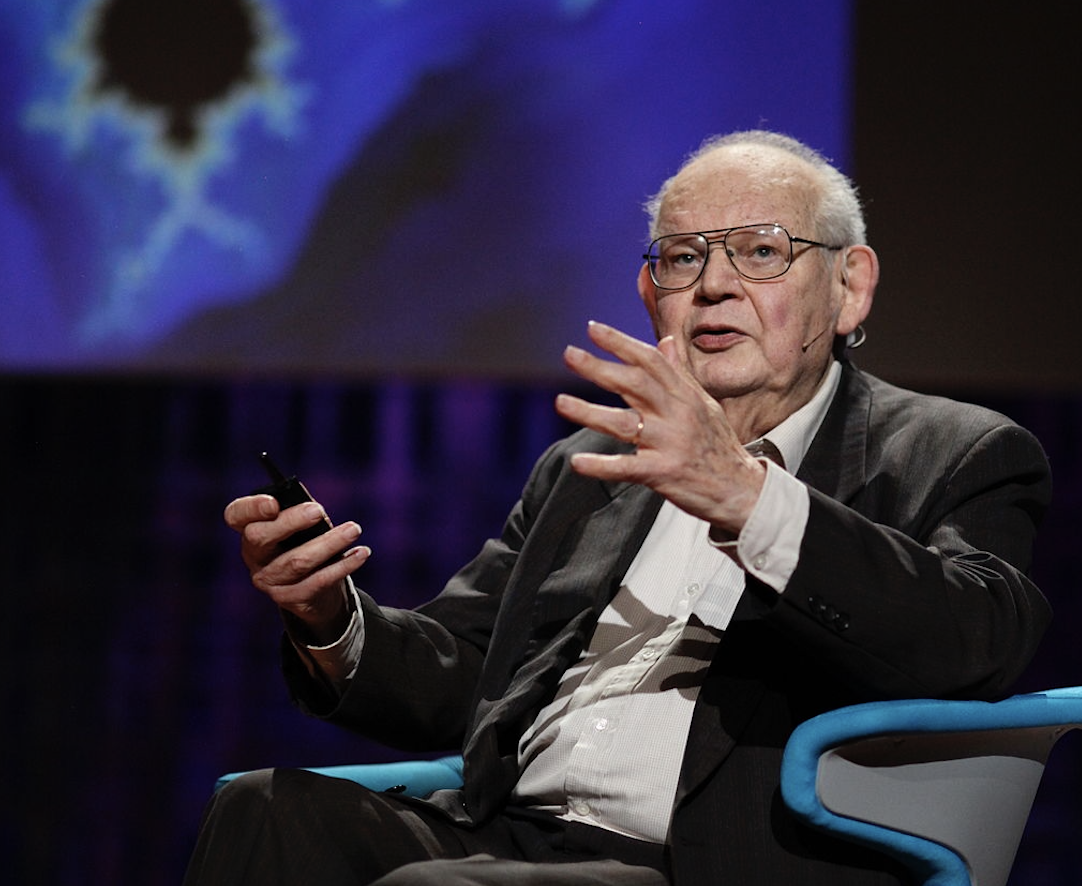
\includegraphics[width=5cm]{./sources/images/mandelbort.png}
\caption{本华·曼德博\textsuperscript{\cite{mandelbort_wiki}}}
\end{minipage}\hfill
\begin{minipage}{0.5\textwidth}
\centering
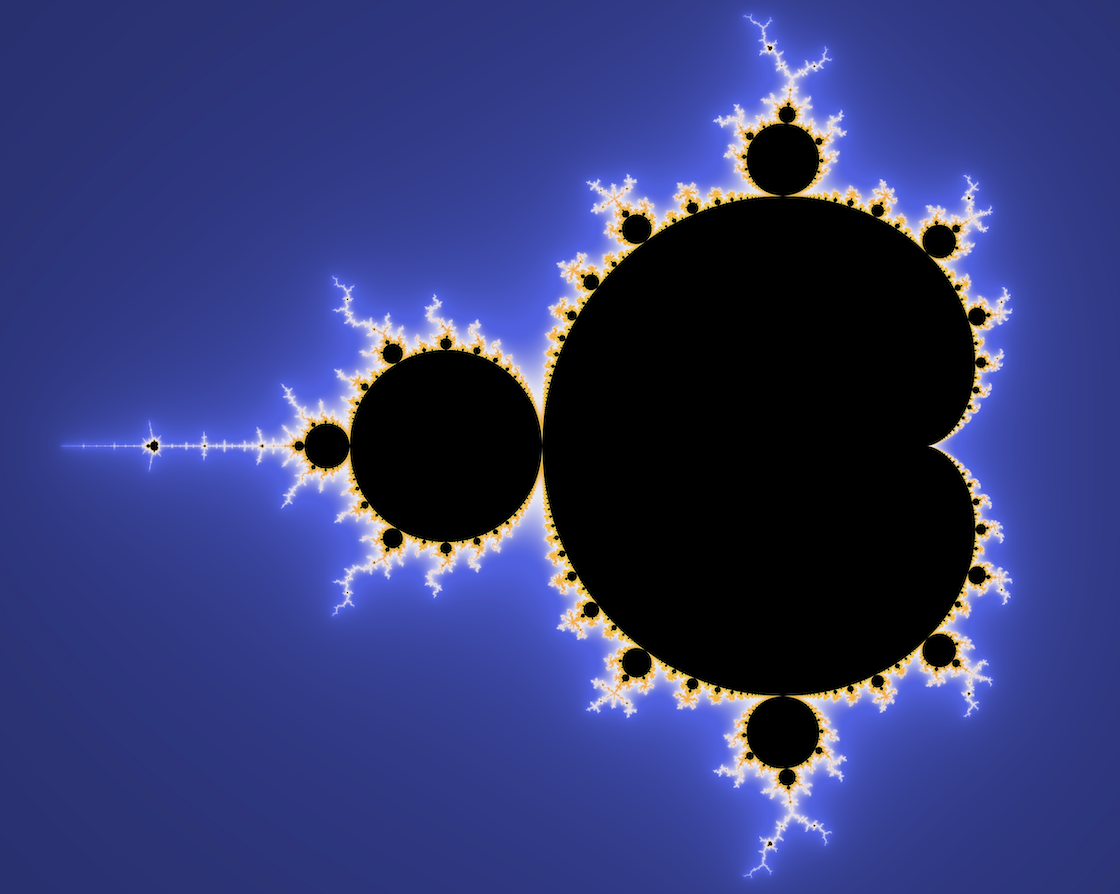
\includegraphics[width=5cm]{./sources/images/set.png}
\caption{曼德博集合图像示例\textsuperscript{\cite{set_pic}}}
\end{minipage}
\end{figure}

曼德博集合是由美国数学家、经济学家本华·曼德博基于其分形理论所刻画的一种在复平面上组成分形的点的集合,其图像轮廓是由几何花边所雕琢的,具有无与伦比的和谐性和精确性,因此也被称为“魔鬼的聚合物”, “上帝的指纹”。\textsuperscript{\cite{mandelbort_wiki}}

事实上,曼德博集合产生于一组非常基础的数学迭代规则,她是分形理论的典型例子,也很好地反映了分形理论的最基本特点,即用分数维度的视角和数学方法描述和研究客观事物。因此,研究曼德博集合图像,可以帮助我们理解数学之于现实空间的美学与应用意义。

\section{背景}
曼德博集起源于复杂的动力学,这是法国数学家Pierre Fatou和Gaston Julia在二十世纪初首次研究的领域。二十世纪下半叶,作为分形之父的曼德博在研究复平面某些变换下具有不变性的朱莉娅集的拓扑基础上提出了曼德博集这一新发现,这种几何重复形式表明一个再简单不过的数学方程也可以产生无限复杂的图像。\textsuperscript{\cite{mandelbort_wiki}}

\section{数学理论}
\subsection{定义\textsuperscript{\cite{set_wiki}}\textsuperscript{\cite{set_wolfram}}}
曼德博集合可以用复二次多项式来定义:
$$f_c(z)=z^2+c$$

其中$c$是一个复数参数。

从$z=0$开始对$f_c(z)$进行迭代:
$$z_{n+1}=z^2_n+c,n=0,1,2,\cdots$$

以此类推,每次迭代的值依序如以下序列所示:
$$(0,f_c(0),f_c(f_c(0)),f_c(f_c(f_c(0)))\cdots)$$

不同的参数$c$可能使迭代值的模逐渐发散到无限大,也可能收敛在有限的区域内。从而,曼德博集合$M$就是使序列不延伸至无限大的所有复数$c$的集合。

当然,曼德尔布罗特集合也可以定义为二次多项式家族的连通性轨迹,而其边界可以定义为该二次多项的分岔轨迹。

\subsection{特性\textsuperscript{\cite{set_wiki}}}
\begin{enumerate}
	\item 自相似性
	\item 局部连接性
	\item 是封闭的紧集
	\item 具有双曲成分
\end{enumerate}

由封闭紧集的特性可以得出,曼德博集合中的点$c$必须满足$|z_n|\le 2$.

\section{算法}
曼德博集合一般用计算机程序计算。对于大多数的分形软件,例如Ultra fractal,内部已经有了比较成熟的例子。

下面的程序是一段伪代码,表达了曼德博集合的计算思路。

\begin{verbatim}
    For Each c in Complex
        repeats = 0
        z = 0
    Do
        z = z^2 + c
        repeats = repeats + 1
    Loop until abs(z) > EscapeRadius or repeats > MaxRepeats  'EscapeRadius可设置为2。
    If repeats > MaxRepeats Then
        Draw c,Black  '如果迭代次数超过MaxRepeats,就将c认定为属于曼德博集合,并设置为黑色。
    Else
        Draw c,color(z,c,repeats)  'color函数用来决定颜色。
    End If
Next
\end{verbatim}

基于上述思路,本文采用了前述数学理论所推导出的关于点是否属于曼德博集合的判断方法,在有限次迭代中近似判定该点的收敛状况。此外,本文实例将生成BMP格式图像,通过将复平面网格化的方法对满足要求的点进行填色绘制。

\section{数值算例}
数值算例的程序基于C++语言进行了完整的封装,只需从外部提供算法的迭代次数$N$、展示图像的中心点$ox$、$oy$及图像半径尺寸$dimension$,即可在images目录下输出目标图像。

在Shell中进入$source$目录并执行$bash run$命令,将获得以下八幅控制参数变量的结果图像:

\textbf{Step.1} 改变迭代次数

\begin{figure}[htb]
\centering
\begin{minipage}{0.48\linewidth}
\centering
\includegraphics[width=\linewidth]{./sources/images/img1_1.bmp}
\caption{N=10,ox=0,oy=0,dimension=3}
\end{minipage}\hfill
\begin{minipage}{0.48\linewidth}
\centering
\includegraphics[width=\linewidth]{./sources/images/img1_2.bmp}
\caption{N=100,ox=0,oy=0,dimension=3}
\end{minipage}
\end{figure}

随着迭代次数增加,图像呈现出更多的细节。

\textbf{Step.2} 改变图像半径尺寸

\begin{figure}[htb]
\centering
\begin{minipage}{0.48\linewidth}
\centering
\includegraphics[width=\linewidth]{./sources/images/img2_1.bmp}
\caption{N=100,ox=0,oy=0,dimension=1.5}
\end{minipage}\hfill
\begin{minipage}{0.48\linewidth}
\centering
\includegraphics[width=\linewidth]{./sources/images/img2_2.bmp}
\caption{N=100,ox=0,oy=0,dimension=0.75}
\end{minipage}
\end{figure}

随着Dimension参数缩小,图像得到相应相对比例的放大。

\textbf{Step.3} 改变中心位置

\begin{figure}[htb]
\centering
\begin{minipage}{0.48\linewidth}
\centering
\includegraphics[width=\linewidth]{./sources/images/img3_1.bmp}
\caption{N=100,ox=0.4,oy=0,dimension=0.75}
\end{minipage}\hfill
\begin{minipage}{0.48\linewidth}
\centering
\includegraphics[width=\linewidth]{./sources/images/img3_2.bmp}
\caption{N=100,ox=0.4,oy=0.4,dimension=0.75}
\end{minipage}
\end{figure}

改变$ox$、$oy$,图像在横纵轴方向上得到了相应的平移。

\textbf{Step.4} 再次提高精度

\begin{figure}[htb]
\centering
\begin{minipage}{0.48\linewidth}
\centering
\includegraphics[width=\linewidth]{./sources/images/img3_1.bmp}
\caption{N=100,ox=0.4,oy=0.4,dimension=0.2}
\end{minipage}\hfill
\begin{minipage}{0.48\linewidth}
\centering
\includegraphics[width=\linewidth]{./sources/images/img3_2.bmp}
\caption{N=1000,ox=0.4,oy=0.4,dimension=0.2}
\end{minipage}
\end{figure}

最后,依次通过缩小Dimension和提高迭代次数,获得更为精细的图像局部。

\section{结论}

通过上述算例,我们详细观察了曼德博集合图像的细节,深入理解了其基本特性与迭代方法等数学理论。如此简洁的算法与其背后的简单公式,同图像本身高度和谐的细节形成了优美的照应。从中,我们可以感知到分形理论为代表的数学工具是如何贯通抽象与具象,把客观理性融于主观美学之中的。

\bibliographystyle{IEEEtran}
\bibliography{ref}

\end{document}